\subsection{Dataset in lingua italiana} \label{ner_ita_data}
\label{sec:ner_dataset_it}
Il dataset utilizzato per l'italiano è stato generato utilizzando training e test set di Named Entity Recognition di EVALITA 2009\footnote{Evalita 2009: \href{https://www.evalita.it/evalita-2009/tasks/entity-recognition/}{https://www.evalita.it/evalita-2009/tasks/entity-recognition/}}. La valutazione è basata sull' \textit{Italian Content Annotation Bank} (I-CAB) dove le entità nominate sono annotate nel formato \textit{IOB} (dove "B-begin" e "I-inside" denotano i token appartenenti a Named Entities e "O-outside" è usato per tutti gli altri token). Per la precisione sono state rigenerate le quattro colonne presenti anche nel dataset in lingua inglese (vedi pagina \pageref{sec:ner_dataset_en}):
\begin{enumerate}
    \item La prima colonna contiene ogni \textbf{token} iniziale della frase.
    \item La seconda il \textbf{POS tag}, secondo il tagset ISST-TANL\footnote{ISST-TANL: \href{http://www.italianlp.it/docs/ISST-TANL-POStagset.pdf}{http://www.italianlp.it/docs/ISST-TANL-POStagset.pdf}}.
    \item  La terza colonna NON contiene il \textbf{chunk sintattico}, che non era previsto nella competizione. Per simmetria con il dataset inglese è stata aggiunta la colonna, ma ogni riga contiene solo il token "\_".
    \item La quarta colonna racchiude il tag della \textbf{named entity} che rispecchia la descrizione del sito, riportata anche sopra.
\end{enumerate}
Il dataset è composto da due file: \textit{I-CAB-evalita09-NER-train\_utf8.tsv} con 11.227 esempi per l’addestramento e \textit{I-CAB-evalita09-NER-test\_utf8.tsv} con 4.136 esempi per il testing.

Le entità presenti nel dataset sono: \textit{persone}, \textit{luoghi}, \textit{organizzazioni} ed entità \textit{geo-politiche}.
\begin{figure}[hbt!]
    \centering
    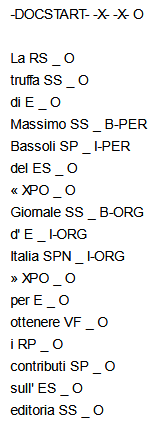
\includegraphics[width=0.17\textwidth]{img/ner_it_dataset.png}
    \caption{Porzione del dataset per NER in lingua italiana}
    \label{fig:ner_it_dataset}
\end{figure}
